\section{Resultados}\label{sec:termpot}

O Termpot (ver Figura \ref{fig:termpot})\footnote{Disponível em \url{https://jahpd.github.io/termpot} e \url{https://www.github.com/jahpd/termpot}.} é um ambiente adaptado segundo uma interpretação do GROOVE, com uma base técnica do \emph{ScriptProcessorNode}. Comandos utilizam a sintaxe da linguagem \emph{coffeescript} \cite{burnham2011coffeescript}\footnote{Disponível em \url{http://coffeescript.org/}.}, que possibilita a improvisação de códigos sonoros com a extensão média de uma linha (ver Código \ref{code:resultado1}). %É interessante notar aqui um princípio de compilação \emph{Just In Time} \cite{aycock_brief_2003}. Antes que uma função de áudio específica seja invocada, o sistema é executado.

\begin{figure}[!h]
\centering
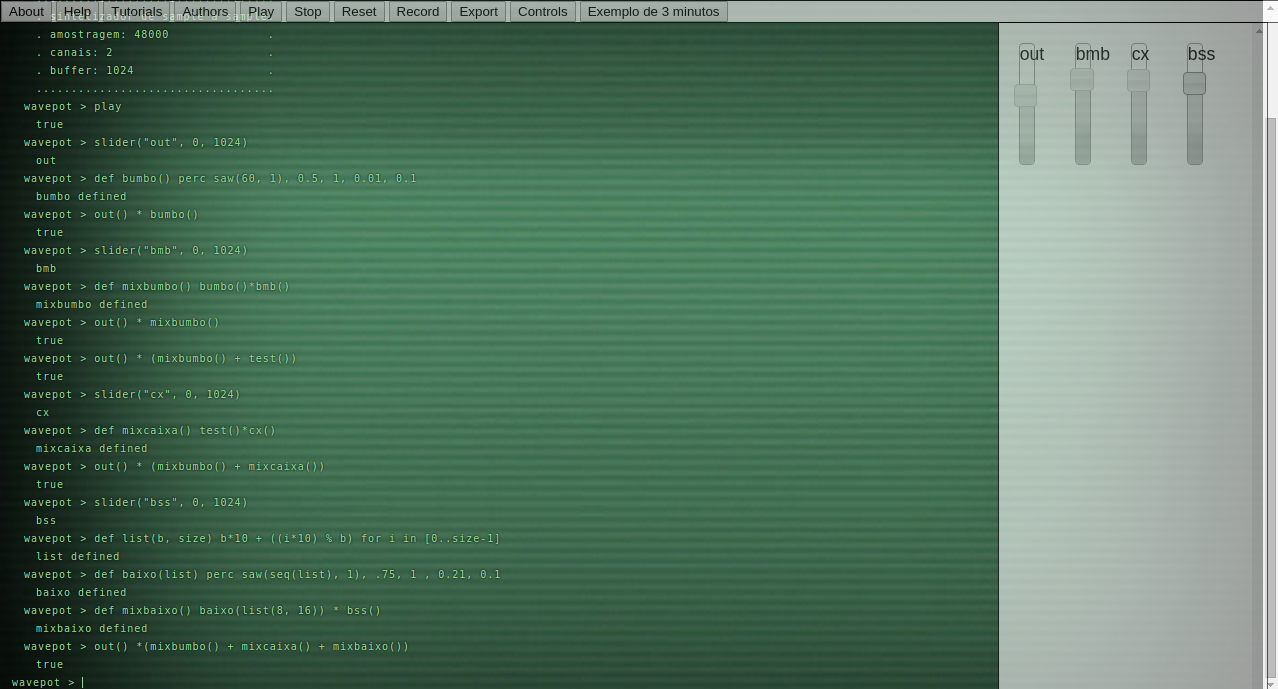
\includegraphics[scale=0.3]{termpot.png}
\caption{Aplicativo \emph{Termpot}. \textbf{Fonte}: autores.}
\label{fig:termpot}
\end{figure}

\begin{listing}
\begin{minted}[linenos,frame=lines,framesep=2mm,fontsize=\scriptsize]{javascript}
$ |                                    (1)
$ wavepot 1024                         (2)
..................................
. sintetizador de sample a sample.     (3) 
. amostragem: 44100              .
. canais: 2                      .
. buffer: 1024                   .
..................................
wavepot > play                         (4)
wavepot > 0.71 * sin 440               (5)
true                                   (6)
\end{minted}
\caption{Mensagem de inicialização do sistema (0). Console do \emph{Termpot} aguardando dados de entrada do improvisador (1). O improvisador inicia o ambiente \emph{wavepot} com um buffer de 1024 amostras por ciclo de DSP (2). Informações diversas do sistema de áudio inicializado (3). O improvisador inicia o processamento de áudio (4). O improvisador define o processamento de áudio (5). O sistema informa que o processamento ocorreu sem problemas (6).}
\label{code:resultado1}
\end{listing}

\subsection*{Criação e edição de funções em tempo de execução}

O \emph{Termpot} é a capaz de definir novas funções em tempo de execução. Do ponto-de-vista dos desenvolvedores, de maneira bastante rápida. Estas funções  podem ser encapsuladas em outras funções. Existem também funções de base, bem como a possibilidade de criar funções especiais, para controle manual. São apresentadas no código \ref{code:resultado}.

\begin{listing}
\begin{minted}[linenos,frame=lines,framesep=2mm,fontsize=\scriptsize]{javascript}
wavepot > def AM(f1, f2) sin f1, sin(f2, 0.5)             (1)
AM defined
wavepot > inspect                                         (2)
funcoes definidas 
tau  tmod  mute  stereo  sin  sin2  saw  ramp  ttri
tri  sqr   pulse noise	 perc test  seq   bpm  nextevent
AM
wavepot > slider "f1", 1, 1025                            (3)
true
wavepot > slider "f2", 1, 1025
true
wavepot > slider "a", 0, 1024            
true
wavepot > AM f1()*1000, f2()*1000                         (4)
true
wavepot > def AM(f1, f2, a) sin f1, sin(f2, a)            (5)
AM redefined
wavepot > AM f1()*1000, f2()*1000, a()                    (6)
true
\end{minted}
\label{code:resultado2}
\caption{Definição de uma nova função, \emph{AM}, que utiliza a função pré-definida \emph{sin} (1). Inspeção das funções definidas no sistema (2). Definição de interfaces gráficas controladoras (3). Execução da função \emph{AM}, controlados por interfaces gráficas (4). Redefinição da função \emph{AM} (5). Reexecução da função \emph{AM}, com um novo controle (6). }
\end{listing}

